\section{Methodology and Evaluation Framework}
\label{sec:methodology}

\subsection{Controlled Grounding Conditions}
To isolate the sources of factual failure, Matibhrom evaluates every prompt under four precisely controlled experimental conditions, formalized as:

\paragraph{Condition $C_0$: Closed-Book (Parametric Memory).} The model receives only the prompt without external documents, requiring reliance strictly on pre-trained parametric weights:
\begin{equation}
    \hat{y}^{(0)} \sim \mathcal{M}_\theta(q)
\end{equation}

\paragraph{Condition $C_1$: Oracle Grounding.} The model is provided the gold passage $e^*$ alongside the prompt:
\begin{equation}
    \hat{y}^{(1)} \sim \mathcal{M}_\theta(q, e^*)
\end{equation}
Condition $C_1$ serves as the theoretical empirical ceiling for reading comprehension, decoupling parametric ignorance from extractive reasoning failure.

\paragraph{Condition $C_2$: Dense RAG with Distractors.} The model receives the top-$k$ retrieved passages ($k=3$) generated by dense vector retrieval over the frozen corpus $\mathcal{D}$:
\begin{equation}
    \mathcal{R}_k(q) = \operatorname{arg\,top-}k_{p \in \mathcal{D}} \; \cos\big(f_{\text{enc}}(q), f_{\text{enc}}(p)\big)
\end{equation}
\begin{equation}
    \hat{y}^{(2)} \sim \mathcal{M}_\theta\big(q, \mathcal{R}_k(q)\big)
\end{equation}
Because $\mathcal{D}$ contains $1,200$ domain-matched distractors, $\mathcal{R}_k(q)$ frequently introduces noisy or irrelevant contexts, modeling realistic production RAG.

\paragraph{Condition $C_3$: Selective Abstention Guardrail.} The model is provided the exact, byte-identical retrieved context $\mathcal{R}_k(q)$ as in $C_2$, but augmented with an explicit negative constraint:
\begin{equation}
    \hat{y}^{(3)} \sim \mathcal{M}_{\theta, \text{abstain}}\big(q, \mathcal{R}_k(q)\big)
\end{equation}
The prompt explicitly mandates: \foreignlanguage{bengali}{\emph{"যদি প্রদত্ত প্রমাণে উত্তর না থাকে, তবে উত্তর অনুমান করবে না; স্পষ্ট করে বলবে 'প্রমাণ অপর্যাপ্ত'।"}} (\emph{"If the provided evidence does not contain the answer, do not guess; state clearly 'Evidence is insufficient'"} / \emph{"proman oporjapto"}).

\begin{figure*}[t]
\centering
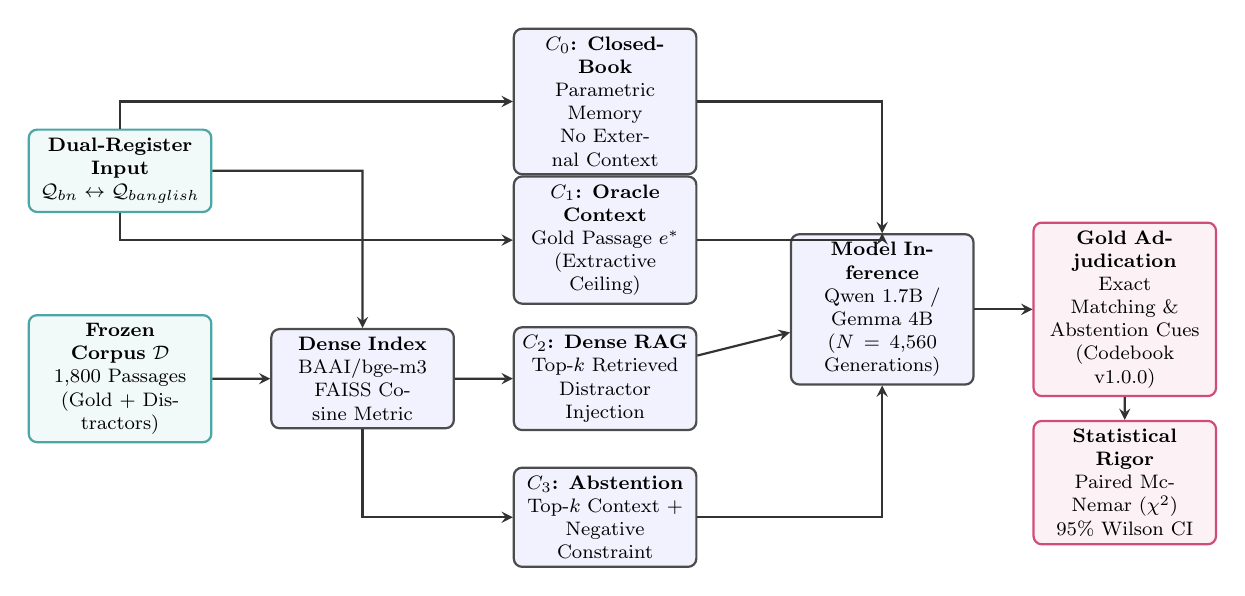
\begin{tikzpicture}[
    scale=0.88, every node/.style={transform shape},
    box/.style={draw=black!70, rounded corners=3pt, thick, fill=blue!5, text width=2.4cm, minimum height=1.1cm, align=center, font=\footnotesize},
    databox/.style={draw=teal!70, rounded corners=3pt, thick, fill=teal!5, text width=2.4cm, minimum height=1.1cm, align=center, font=\footnotesize},
    evalbox/.style={draw=purple!70, rounded corners=3pt, thick, fill=purple!5, text width=2.4cm, minimum height=1.1cm, align=center, font=\footnotesize},
    arrow/.style={->, >=stealth, thick, color=black!80}
]
    % Inputs
    \node[databox] (query) at (0, 2) {\textbf{Dual-Register Input}\\$\mathcal{Q}_{\text{bn}} \leftrightarrow \mathcal{Q}_{\text{banglish}}$};
    \node[databox] (corpus) at (0, -1) {\textbf{Frozen Corpus $\mathcal{D}$}\\1,800 Passages\\(Gold + Distractors)};
    
    % Retriever
    \node[box] (retriever) at (3.5, -1) {\textbf{Dense Index}\\BAAI/bge-m3\\FAISS Cosine Metric};
    
    % Conditions
    \node[box] (c0) at (7, 3) {\textbf{$C_0$: Closed-Book}\\Parametric Memory\\No External Context};
    \node[box] (c1) at (7, 1) {\textbf{$C_1$: Oracle Context}\\Gold Passage $e^*$\\(Extractive Ceiling)};
    \node[box] (c2) at (7, -1) {\textbf{$C_2$: Dense RAG}\\Top-$k$ Retrieved\\Distractor Injection};
    \node[box] (c3) at (7, -3) {\textbf{$C_3$: Abstention}\\Top-$k$ Context +\\Negative Constraint};
    
    % Model Generation
    \node[box] (model) at (11, 0) {\textbf{Model Inference}\\Qwen 1.7B / Gemma 4B\\($N=4{,}560$ Generations)};
    
    % Evaluation
    \node[evalbox] (adjudication) at (14.5, 0) {\textbf{Gold Adjudication}\\Exact Matching \&\\Abstention Cues\\(Codebook v1.0.0)};
    \node[evalbox] (stats) at (14.5, -2.5) {\textbf{Statistical Rigor}\\Paired McNemar ($\chi^2$)\\95\% Wilson CI};

    % Arrows
    \draw[arrow] (corpus) -- (retriever);
    \draw[arrow] (query) |- (c0);
    \draw[arrow] (query) |- (c1);
    \draw[arrow] (query) -- (3.5, 2) -- (retriever);
    \draw[arrow] (retriever) -- (c2);
    \draw[arrow] (retriever) |- (c3);
    
    \draw[arrow] (c0) -| (model);
    \draw[arrow] (c1) -| (model);
    \draw[arrow] (c2) -- (model);
    \draw[arrow] (c3) -| (model);
    
    \draw[arrow] (model) -- (adjudication);
    \draw[arrow] (adjudication) -- (stats);
\end{tikzpicture}
\caption{End-to-End Matibhrom Experimental Framework: From matched dual-register queries and frozen dense retrieval indexing to 4-condition generation, gold-verified adjudication, and paired statistical testing.}
\label{fig:methodology_framework}
\end{figure*}

\subsection{Formal Evaluation Metrics}
For a sample of $N$ evaluated generations, every output $\hat{y}_i$ is adjudicated into correctness $c_i \in \{\text{correct}, \text{partially}, \text{incorrect}\}$, hallucination indicator $h_i \in \{\text{yes}, \text{no}\}$, error category $\epsilon_i \in \{\text{H1}, \dots, \text{H5}, \text{A}, \text{R}, \text{none}\}$, and abstention status $b_i \in \{\text{none}, \text{appropriate}, \text{unnecessary}\}$. We compute four primary metrics:

\paragraph{1. Hallucination Rate ($\mathcal{H}$):} The proportion of generations containing factually fabricated or contradictory claims:
\begin{equation}
    \mathcal{H} = \frac{1}{N} \sum_{i=1}^N \mathbf{1}[h_i = \text{yes}]
    \label{eq:hallucination_rate}
\end{equation}

\paragraph{2. Substantive Coverage ($\mathcal{C}$):} The fraction of queries for which the model attempts a substantive answer rather than refusing or abstaining:
\begin{equation}
    \mathcal{C} = \frac{1}{N} \sum_{i=1}^N \mathbf{1}[b_i = \text{none} \land \epsilon_i \neq \text{R}]
    \label{eq:coverage}
\end{equation}

\paragraph{3. Selective Accuracy ($\mathcal{A}_{\text{sel}}$):} Accuracy computed strictly over the subset of answered (non-abstained) queries:
\begin{equation}
    \mathcal{A}_{\text{sel}} = \frac{\sum_{i: b_i = \text{none} \land \epsilon_i \neq \text{R}} \big(\mathbf{1}[c_i = \text{correct}] + 0.5 \cdot \mathbf{1}[c_i = \text{partially}]\big)}{\sum_{i=1}^N \mathbf{1}[b_i = \text{none} \land \epsilon_i \neq \text{R}]}
    \label{eq:selective_accuracy}
\end{equation}

\paragraph{4. Abstention Rate ($\mathcal{B}$):} The fraction of queries where the model explicitly invokes abstention or refusal:
\begin{equation}
    \mathcal{B} = \frac{1}{N} \sum_{i=1}^N \mathbf{1}[b_i \neq \text{none}]
    \label{eq:abstention_rate}
\end{equation}

\subsection{Statistical Significance and Hypothesis Testing}
To establish empirical significance without making unwarranted parametric distributional assumptions, all pairwise comparisons are evaluated using paired McNemar tests~\citep{mcnemar1947note} with Edwards' continuity correction:
\begin{equation}
    \chi^2 = \frac{\big(|b - c| - 1\big)^2}{b + c}, \quad p = \operatorname{Pr}(\chi^2_1 \ge \chi^2)
    \label{eq:mcnemar}
\end{equation}
where $b$ is the count of items where Condition 1 hallucinates and Condition 2 does not, and $c$ is the converse. In addition, for all reported metrics, we estimate 95\% confidence intervals via non-parametric bootstrapping with $B = 1,000$ resamples.

\subsection{Evaluation Algorithm}
Algorithm~\ref{alg:matibhrom_pipeline} outlines the complete evaluation and adjudication protocol.

\begin{algorithm}[t]
\caption{Matibhrom Multi-Condition Evaluation Protocol}
\label{alg:matibhrom_pipeline}
\begin{algorithmic}[1]
\Require Base items $\mathcal{I}$, Corpus $\mathcal{D}$, Embedding model $f_{\text{enc}}$, LLMs $\mathcal{M}_\theta$, Conditions $\mathcal{C} = \{C_0, C_1, C_2, C_3\}$, Registers $\mathcal{L} = \{\text{bn}, \text{banglish}\}$
\Ensure Evaluation metrics $\mathcal{H}, \mathcal{C}, \mathcal{A}_{\text{sel}}, \mathcal{B}$ with bootstrap 95\% CIs and McNemar tests
\State Index corpus passages: $\mathbf{V}_{\mathcal{D}} \leftarrow \{f_{\text{enc}}(p) \mid p \in \mathcal{D}\}$ into FAISS
\For{each model $\mathcal{M}_\theta$}
    \For{each item $i \in \mathcal{I}$, register $l \in \mathcal{L}$, condition $c \in \mathcal{C}$}
        \State Formulate query $q \leftarrow i.\mathcal{Q}_l$
        \If{$c = C_0$}
            \State $\hat{y} \leftarrow \mathcal{M}_\theta(q)$
        \ElsIf{$c = C_1$}
            \State $\hat{y} \leftarrow \mathcal{M}_\theta(q, i.e^*)$
        \ElsIf{$c = C_2$}
            \State $\mathcal{R}_k(q) \leftarrow \operatorname{Top-}k(\cos(f_{\text{enc}}(q), \mathbf{V}_{\mathcal{D}}))$
            \State $\hat{y} \leftarrow \mathcal{M}_\theta(q, \mathcal{R}_k(q))$
        \ElsIf{$c = C_3$}
            \State $\mathcal{R}_k(q) \leftarrow \operatorname{Top-}k(\cos(f_{\text{enc}}(q), \mathbf{V}_{\mathcal{D}}))$
            \State $\hat{y} \leftarrow \mathcal{M}_{\theta, \text{abstain}}(q, \mathcal{R}_k(q))$
        \EndIf
        \State Record generation $\hat{y}$ to atomic storage
    \EndFor
\EndFor
\State \textbf{Adjudication:} Match $\hat{y}$ against gold answer $i.\mathcal{A}^*$ and abstention cues
\State Compute $\mathcal{H}, \mathcal{C}, \mathcal{A}_{\text{sel}}, \mathcal{B}$ via Eqs.~(\ref{eq:hallucination_rate})--(\ref{eq:abstention_rate})
\State Calculate bootstrap 95\% CIs ($B=1,000$) and McNemar $\chi^2$ via Eq.~(\ref{eq:mcnemar})
\end{algorithmic}
\end{algorithm}
